\documentclass{article}
\usepackage{amssymb}
\usepackage{amsmath}
\usepackage{graphicx}
\usepackage{tikz}
\usetikzlibrary{arrows}
%Week 1

\begin{document}
\begin{center}
\textbf{\huge{Week 1}}
\end{center}
\section{Communication Theory}

Communication theory is a field of information theory and mathematics that studies the technical process of information.
Communication theory consists of:
\begin{itemize}
    \item Analyzing real world communication systems using structured thinking or mathematics.
    \item Synthesizing real world communication systems from mathematics.
\end{itemize}

\section{Signals}
Signals are defined to be a function that conveys information about a phenomenon.
They can also be said to be a medium which carry information relevant to a reciever.

Electromagnetic wave, voltage or current, digital signals carrying information are some examples of signals.

\subsection{Are there any non-time based signals?}
\begin{itemize}
    \item Images: They are represented as a combination of  monochrome images in three primary colors.
    $$ Image: \mathbb{R}^2 \rightarrow \{ R, G, B\}$$
    \item Temperature at various points in a room.
    $$ Temperature:\mathbb{R}^3 \rightarrow K \quad(or\; Celsius)$$
    \item Videos:  A video signal is a sequence of images.
    \item Text or a page in a book.
\end{itemize}

\section{Communication}
Communication is the process of exchanging information. Transmission, reception and reconstruction of the transmitted signal take place in this process.
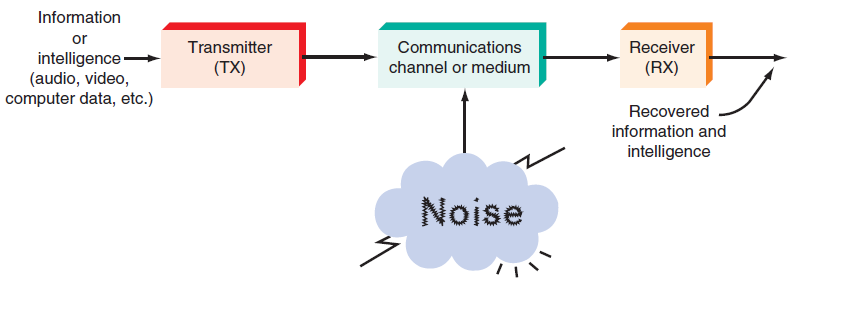
\includegraphics[width=\textwidth]{ptp.png}

Channel: Separates the source and reciever and is not directly under our control.
This leads to some disturbances or imperfections in the channel, which is called noise.

\subsection{Transmitter}
The first step in sending a message is to convert it into electronic form suitable for transmission. The transmitter consists of various components designed to convert the electrical signal to a signal for sending it through the medium.

$$\fbox{Source} \xrightarrow{info.} \fbox{Channel Coding/Amplification/Modulation/Antenna} \rightarrow \fbox {Channel} $$

The transmitter is also called TX or TRX.

\subsection{Reciever}

\tikzstyle{int}=[draw, minimum size=2em]
\tikzstyle{init} = [pin edge={to-,thin,black}]
\begin{tikzpicture}[node distance=6cm,auto,>=latex']
    \node [int] (a) {Detect/estimate signal};
    \node (b) [left of=a,node distance=5cm, coordinate] {a};
    \node [int] (c) [right of=a] {Extract info.};
    \node [coordinate] (end) [right of=c, node distance=2cm]{};
    \path[->] (b) edge node {Noisy TX signal} (a);
    \path[->] (a) edge node {Channel decoding} (c);
    \draw[->] (c) edge node {} (end) ;
\end{tikzpicture}
\newline
A receiver is a collection of electronic components and circuits that accepts the transmitted message from the channel and converts it back to an understandable form.
The dectection and estimation step is called `demodulation'.

Channel coding and decoding is mainly used in digital communication systems. The reciever is called RX.

\subsection{Features of a good communication system}
\begin{itemize}
    \item Low degradation in quality of original signal, called high fidelity.
    \item Quick reception of information, called high rate communication.
        (in digital comms., this happens via intelligent modulation, power control)
    \item Time delay between transmission and communication should be small, called latency. (eg: high latency required in video streams but not for downloads)
\end{itemize}

\subsection{Modes of Communication}
\begin{enumerate}
    \item Point-to-point communication, in which the communication process takes place over a link between a single transmitter and a receiver. eg: Wired phone call.
    \item Broadcasting, which involves the use of a single  transmitter and multiple receivers. eg: Radio/TV broadcast, wi-fi, wireless cellular downlink
    \begin{itemize}
        \item Multiple access channel, consists of multiple transmitters and a single reciever. eg: Cellular uplink.
    \end{itemize}
\end{enumerate}

\section{Information}

\subsection{What is information?}
    Information is often thought of as the resolution of uncertainity. It can also mean the arrangement of particles.

    Say that $X$ is a random quantity representing the signal of interest (at some point in time or space).

$X \in \{0,1\}$ and it can take value $0$ with a probability of $p$ and value $1$ with probability $1-p$. This statement is a general abstraction of many different real-world scenarios.
$X$ is called a random variable, while 0 and 1 together form the sample space.

How do we find the information-content (or ``surprise'', ``average uncertainty'') in X?

The information content(surprise) is inversely proportional to the probability that the event occurs. i.e.
$$ Info.\; content\; in \;event \;``X=0" \propto \frac{1}{P(X=0)}$$

Our goal is to assign a function to the above `information content'.

Suppose $X_1\, \&\, X_2$ are independant random variables and $x_1, x_2$ are some values. Then
$$ P(X_1=x_1,X_2=x_2)=P(X_1=x_1)\times P(X_2=x_2)$$

We expect the joint information content in $X_1\, \&\, X_2$ to be the sum of the individual information contents.(as product is being converted to a sum, the log function is a good choice)

The information content in the event $X=x$ is $\log( {\frac{1}{P(X=x)})}$.

\subsection{Entropy}

The average (or expected) information content for a random variable $X$, with possible outcomes $x_1, \cdots, x_n$, which occur with probability $P(x_1),\cdots, P(x_n)$ is defined as:

$$ H(X) :=- \sum_{i=1}^{n} P(x_i) \log P(x_i)$$

$H(X)$ is called the entropy of X. Entropy in information theory is directly analogous to the entropy in statistical thermodynamics.

\subsubsection{Lemma}
Suppose $x_1 \in \mathcal{X}_1\, \&\; x_2 \in \mathcal{X}_2$ are \textbf{independant} random variables. Then,
$$ H(x_1,\;x_2)=H(x_1)+H(x_2)$$






\end{document}
